\chapter{PCB Design}
Once the components were chosen and there schematics drawn up. Altium Designer was then used to create the PCB design of the servo motor controller that could then be converted into a format that the PCB manufacturers, TraX, can then use to create the PCB. The board was designed in several stages.

\section{Schematic}
The first step in designing the PCB on was to create each of the designed schematics in Altium. All the necessary pins, net labels were connected up for each component. The schematics can be seen in the following pages.
\begin{figure}[H]
\centering
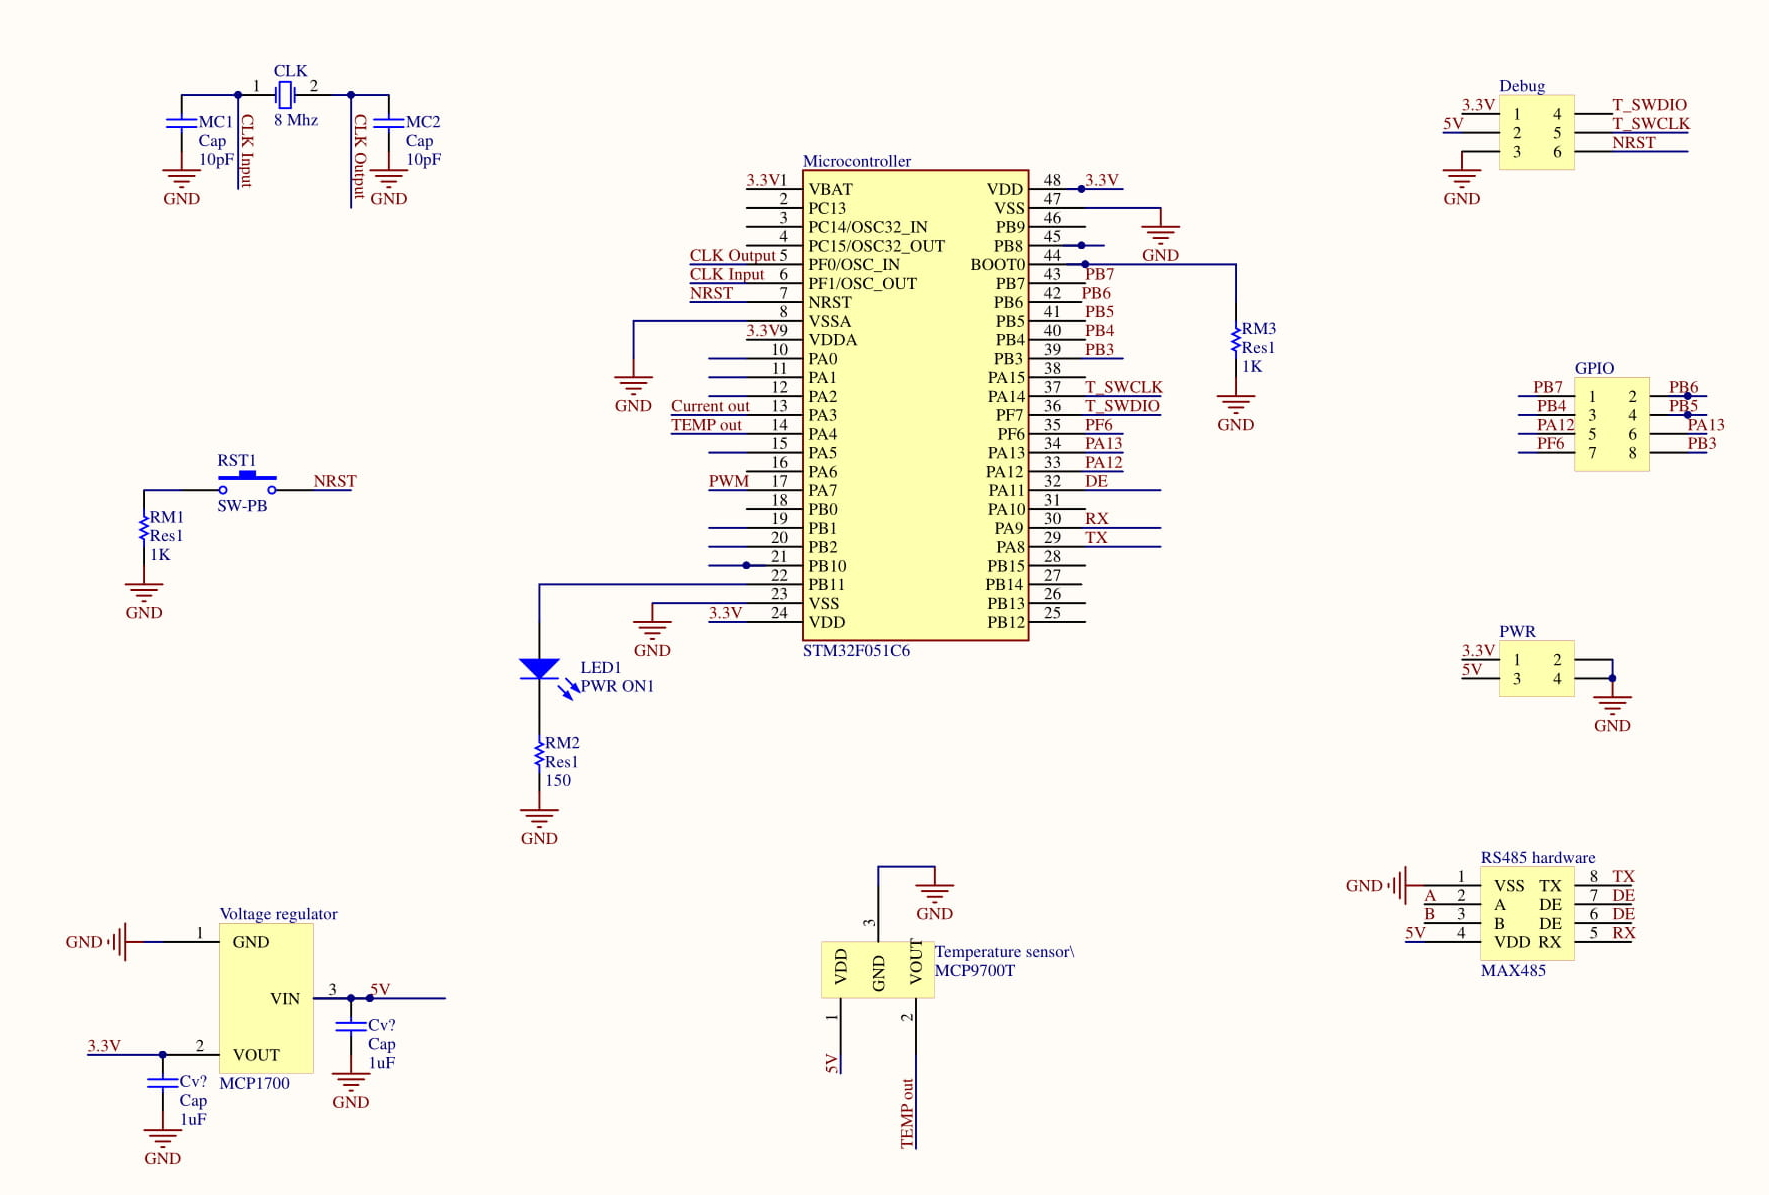
\includegraphics[width=1\textwidth]{Microsch.jpg}
\vspace{-5mm}
\caption{Microcontroller and components schematic}
\end{figure} 

\newpage
\begin{figure}[H]
\centering
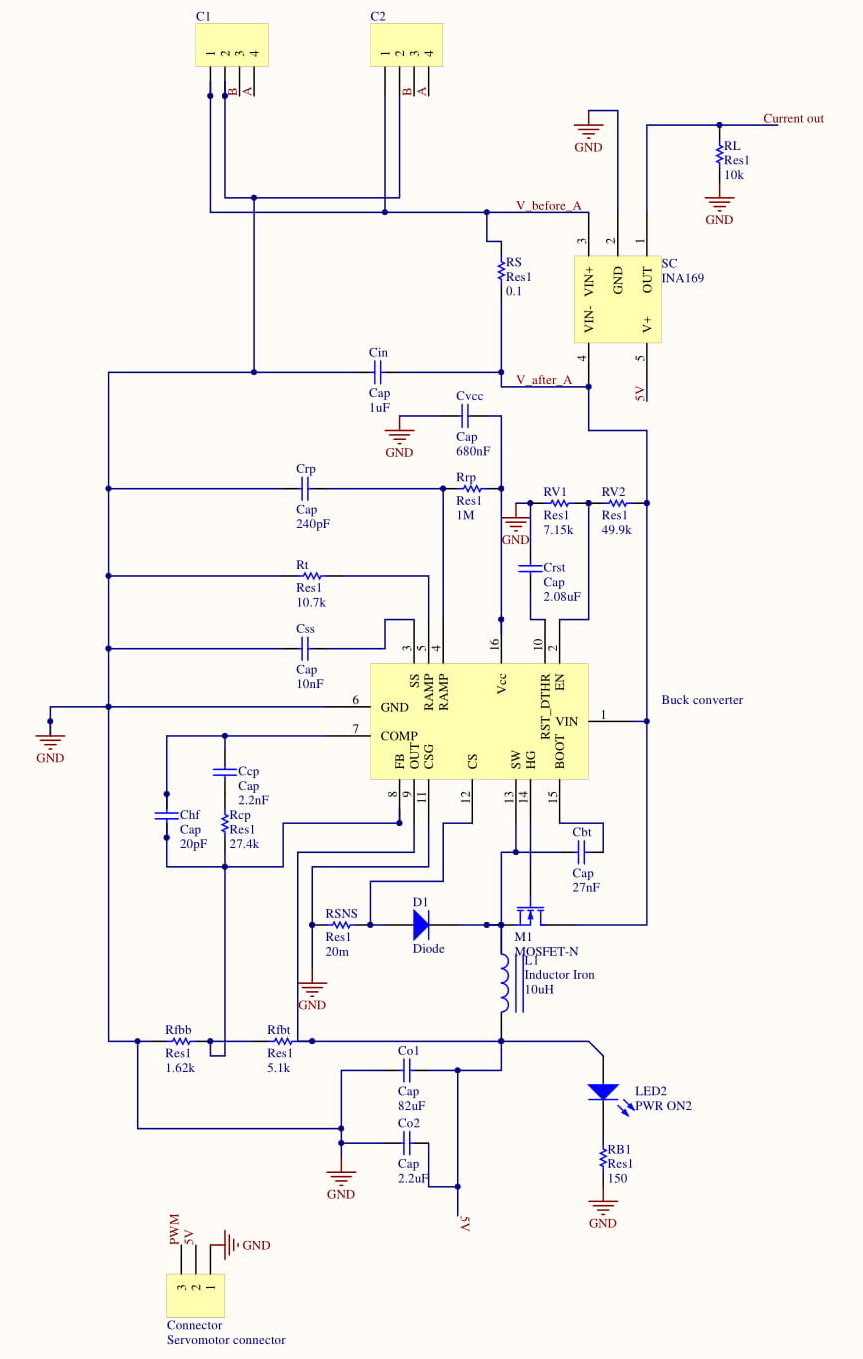
\includegraphics[width=0.85\textwidth]{bucksch.jpg}
\caption{Buck converter schematic}
\end{figure} 

\newpage
\section{Parts and footprints}
Each component chosen will have an associated PCB footprint, where the solder pads and through connectors may be soldered. Most resistors, capacitors and inductors come in various standard package sizes, but other components such as the MOSFET or buck converter will have their own unique footprint. For these components the parts and their footprints had to be specifically made using measurements from the associated data sheet. 

First each component needed to be designed in an Altium library. This is where the pin numbers and outputs are allocated. 
\hspace{5mm}
\begin{figure}[H]
\centering
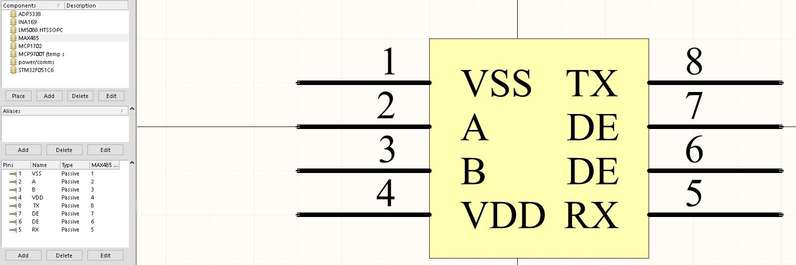
\includegraphics[width=0.8\textwidth]{library.JPG}
\caption{Creating a component}
\label{fig:model}
\end{figure} 

Each components footprint was also then created. This is where the actual solder pad for each pin is created.
\hspace{5mm}
\begin{figure}[H]
\centering
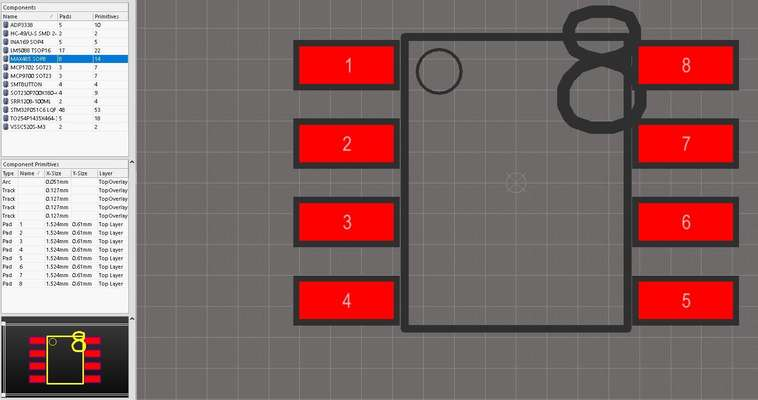
\includegraphics[width=0.7\textwidth]{footprints.JPG}
\caption{Creating a footprint}
\label{fig:model}
\end{figure} 

\newpage
\section{Board optimisation}

Once the schematic was designed, and all the components and their footprints were either found in the free Altium libraries (Altium Vault) or created, a model of the PCB can be created. At this point the components can be placed and any physical specifications of the PCB can be defined. 

In an initial design, the placement of components and the routing of the tracks had been done in a messy and inefficient way.  The tracks created between components looped around other components or obstacles when attempting to take the shortest route. Laying tracks like this can lead to stray inductances, more importantly, the tracks between all the components were the same width and did not take current requirements into account which can lead to the tracks breaking and causing damage to the PCB. No ground plain had been used and this added to additional ground tracks running across the PCB. 

\vspace{-5mm}
\subsection{Track parameters}    
The buck converter will be supplying all the current to the servo motor as well as to the rest of the components on the board board. The standard track width automatically set on Altium Designer is 0.25mm, which is much too thin to carry up the 4 Amps that the buck converter was designed to output. Using the following formula the necessary trace width was calculated \cite{tracewidth}.
\vspace{-2mm}
\begin{center}
\Large
$ Width = \frac{(Current[Amps]/(k*(Temprise[\degree C]^b)^(1/c)))} {(Thickness[oz]*1.378[mils/oz]) }$

\begin{table}[H]
\centering
  \begin{tabular}{cl}
    \textbf{Where :}\\
    & k = 0.024 \\
    & b = 0.044\\
    & c = 0.725\\
    & Current  = 4 A\\
    & Temprise = 10 \degree C\\
    & Thickness = 0.725 mm\\
   
  \end{tabular}
\end{table}
\end{center}
\vspace{-5mm}
it was calculated that the track width would need to be roughly 2.8 mm, so a safe width of 4 mm was chosen for all the tracks that would be carrying high current. The lower current pins were given a track width of 0.8 mm.


\subsection{Component positioning}
\vspace{-5mm}
The buck converters positioning relative to the rest of the components, especially the microcontroller, is an important factor. Switch mode supplies tend to generate a switching noise at the switching frequency which is generally between 500kHz and 3MHz \cite{noise}. This was solved in two ways. First was to separate the buck converter from the microcontroller by putting the two devices on opposite sides of the board. The other  was to create a ground plane on the top and bottom of the board. The ground plane would would then ground any stray EM signals that will be created. This would also neaten up the board by reducing the number of ground tracks that would be otherwise required. This was achieved using Altium Designers Polygon pours option setting.

Once the buck converter had been placed, the next few parts that needed to be positioned were the current and temperature sensors, the 3.3v regulator, and the MAX485. All of these were relatively straight forward, keeping in mind that the MAX485 needed to be as close to the micro as possible as to reduce any possible noise. Any input and output pins as well as the reset button and any LED's were then positioned in such a way as to optimise the functioning of the board as well as to keep it as compact as possible.

\vspace{-5mm}
\subsubsection{Optimised layout}    
\vspace{-5mm}
The layout for the optimised PCB can be seen in Figure 3.18 with each individual components being highlighted.
\begin{figure}[H]
\centering
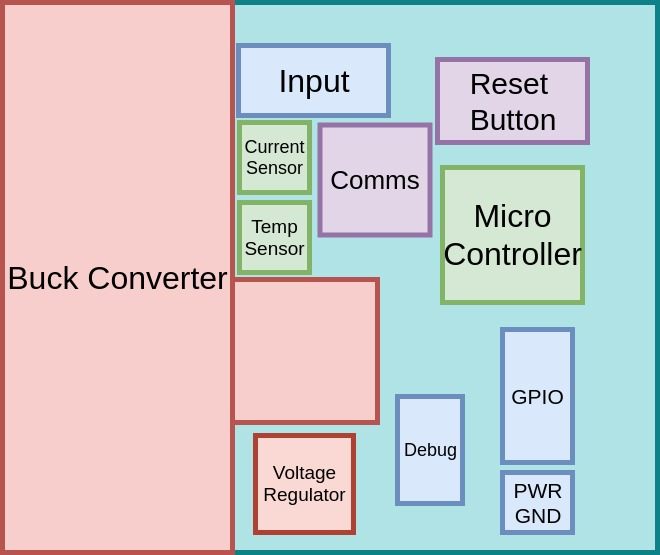
\includegraphics[width=0.6\textwidth]{PCB_breakdown.jpg}
\caption{Optimised PCB layout}
\end{figure} 
\vspace{-5mm}

\subsection{Final Design}
\vspace{-5mm}
The final schematic for the PCB design can be seen below in Figure 5.6. The top(red) and bottom(blue) layer tracks and pads can be seen. The top and bottom ground planes were removed for this schematic to make the tracks more visible.
\vspace{-2mm}
\begin{figure}[H]
\centering
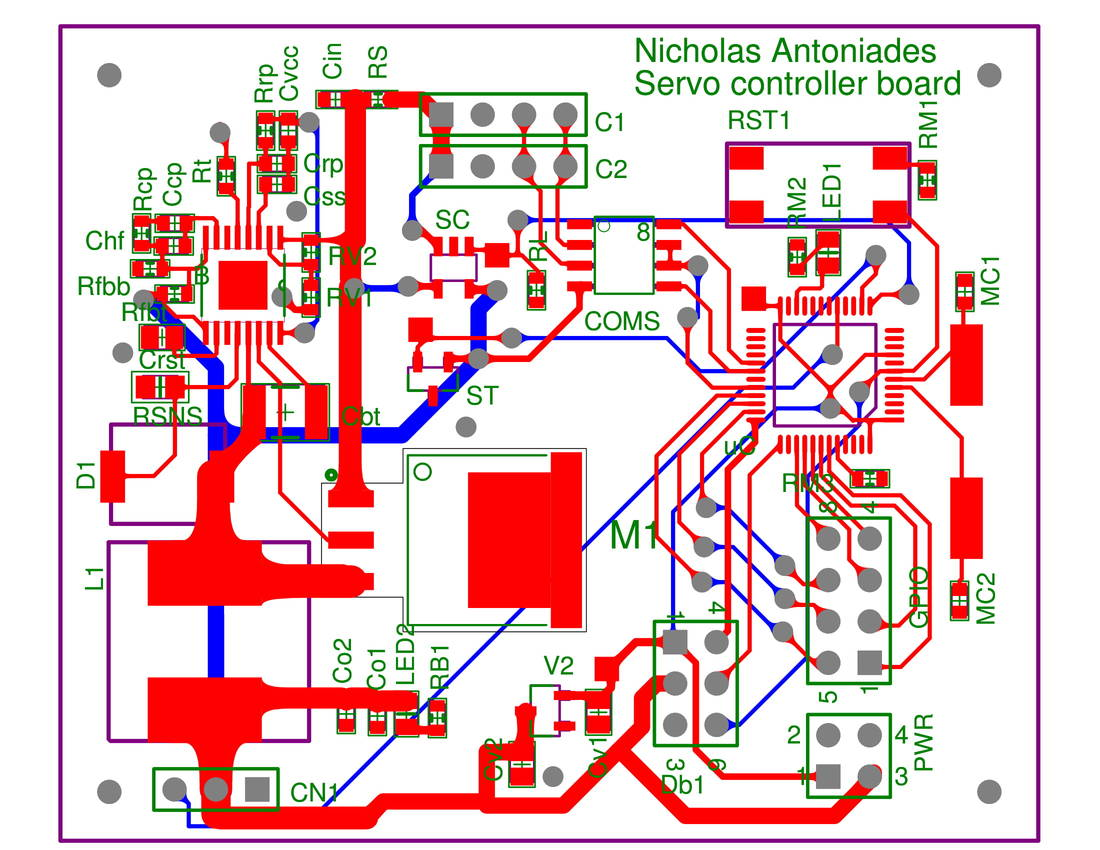
\includegraphics[width=0.7\textwidth]{Final_PCB.jpg}
\caption{Final PCB design}
\end{figure} 
\vspace{-10mm}
Once the final design was completed it was exported to the Gerber format and sent of to Trax, where the actual PCB was manufactured.

\vspace{-10mm}
\subsection{Component List}
\begin{table}[H]
    \vspace{-5mm}
    \centering
    \scriptsize{
    \begin{tabular}{|l|l|l|l|l|l|}
         \hline
         \textbf{\underline{Buck converter}}& \underline{R101.82} & \textbf{\underline{Micro}}  & \underline{R65.66 }& \textbf{\underline{Current sensor}}&\underline{R38.88} \\
         $R_{rp}$ = 1M\ohm      &0.63&   $R_{M1}$ = 1k\ohm   &0.62&   $R_{RL}$ = 10k\ohm      &0.63\\
         $R_{t}$ = 10.7k\ohm    &0.64&   $R_{M2}$ = 150\ohm  &0.66&  $R_{RS}$ = 0.1\ohm      &4.85\\       
         $R_{V1}$ = 7.15k\ohm   &0.66&   $R_{M3}$ = 1k\ohm   &0.67&   SC = INA169             &33.40\\ 
         $R_{V2}$ = 49.9k\ohm   &0.73&                       &&                           &\\
         $R_{cp}$ = 27.4k\ohm   &0..85& $C_{MC1}$ = 10pF &2.35&  \textbf{\underline{Temperature sensor}}&\underline{R3.61}\\
         $R_{RSNS}$ = 20M\ohm   &0.68&   $C_{MC2}$ = 10pF    &2.35&   ST = MCP9700T           &3.61\\     
         $R_{fbt}$ = 5.1k\ohm   &0.68&                       &&                           &\\
         $R_{B1}$ = 150\ohm     &0.62&   uC = STM32F051C6    &35.17&   \textbf{\underline{RS485}}&\underline{R72.11}\\     
                                &&   8mHz crystal           &4.83&   COMS = MAX485           &72.11\\
         $C_{hf}$ = 20pF        &0.56&   LED                 &5.23&                           &\\   
         $C_{cp}$ = 2.2nF       &0.32&   SMD push button     &13.78& \textbf{\underline{Voltage regulator}} &\underline{R8.28}\\ 
         $C_{bt}$ = 27nF        &0.61&                      &&    V2 = MCP1700T       &8.28\\  
         $C_{o1}$ = 82uF        &5.23&                      &&                           &\\                                          
         $C_{o2}$ = 2.2uF       &1.53&                      &&                           &\\                                              
         D1 = VSSC520S-M3       &8.45&                      &&                           &\\   
         M1 = IPD50N10S3l16  &14.67&                       &&                           &\\                                          
         L1 = 10uH              &10.12&                       &&                           &\\    
         B1 = LM5088            &54.52&                       &&                           &\\  
         \hline
         \textbf{Total cost: R290.36}&&&&&\\
         \hline
    \end{tabular}}
    \caption{Component list}
\end{table}
\vspace{-10mm}
